%%%%%%%%%%%%%%%%%%%%%%%%%%%%%%%%%%%%%%%%%
% Beamer Presentation
% LaTeX Template
% Version 1.0 (10/11/12)
%
% This template has been downloaded from:
% http://www.LaTeXTemplates.com
%
% License:
% CC BY-NC-SA 3.0 (http://creativecommons.org/licenses/by-nc-sa/3.0/)
%
%%%%%%%%%%%%%%%%%%%%%%%%%%%%%%%%%%%%%%%%%

%----------------------------------------------------------------------------------------
%	PACKAGES AND THEMES
%----------------------------------------------------------------------------------------

\documentclass{beamer}

\mode<presentation> {

% The Beamer class comes with a number of default slide themes
% which change the colors and layouts of slides. Below this is a list
% of all the themes, uncomment each in turn to see what they look like.

\usetheme{default}
%\usetheme{AnnArbor}
%\usetheme{Antibes}
%\usetheme{Bergen}
%\usetheme{Berkeley}
%\usetheme{Berlin}
%\usetheme{Boadilla}
%\usetheme{CambridgeUS}
%\usetheme{Copenhagen}
%\usetheme{Darmstadt}
%\usetheme{Dresden}
%\usetheme{Frankfurt}
%\usetheme{Goettingen}
%\usetheme{Hannover}
%\usetheme{Ilmenau}
%\usetheme{JuanLesPins}
%\usetheme{Luebeck}
%\usetheme{Madrid}
%\usetheme{Malmoe}
%\usetheme{Marburg}
%\usetheme{Montpellier}
%\usetheme{PaloAlto}
%\usetheme{Pittsburgh}
%\usetheme{Rochester}
%\usetheme{Singapore}
%\usetheme{Szeged}
%\usetheme{Warsaw}

% As well as themes, the Beamer class has a number of color themes
% for any slide theme. Uncomment each of these in turn to see how it
% changes the colors of your current slide theme.

%\usecolortheme{albatross}
%\usecolortheme{beaver}
%\usecolortheme{beetle}
%\usecolortheme{crane}
%\usecolortheme{dolphin}
%\usecolortheme{dove}
%\usecolortheme{fly}
%\usecolortheme{lily}
%\usecolortheme{orchid}
%\usecolortheme{rose}
%\usecolortheme{seagull}
%\usecolortheme{seahorse}
%\usecolortheme{whale}
%\usecolortheme{wolverine}

%\setbeamertemplate{footline} % To remove the footer line in all slides uncomment this line
%\setbeamertemplate{footline}[page number] % To replace the footer line in all slides with a simple slide count uncomment this line

%\setbeamertemplate{navigation symbols}{} % To remove the navigation symbols from the bottom of all slides uncomment this line
}

\usepackage{graphicx} % Allows including images
\usepackage{booktabs} % Allows the use of \toprule, \midrule and \bottomrule in tables
\usepackage{amsmath}
\usepackage{xcolor}
\usepackage{graphicx}
\usepackage{ragged2e}
%\usepackage[style=authoryear,maxcitenames=1,maxnames = 50]{biblatex}
\usepackage{forest}
\usepackage{tikz}
\usepackage{tikz-cd}
\usepackage{changepage}


% Beamer theme font
\usefonttheme{structurebold} % bold titles

%\renewcommand*{\nameyeardelim}{\addcomma\addspace}

%\addbibresource{support/MHMMpresbib.bib}

%\setbeamertemplate{bibliography item}[text]

% \setbeamersize{text margin left=3mm,text margin right=3mm} 

%----------------------------------------------------------------------------------------
%	TITLE PAGE
%----------------------------------------------------------------------------------------

\title[]{Practical Concerns for Estimating Mixed Hidden Markov Models with an Application to Actigraphy Data} % The short title appears at the bottom of every slide, the full title is only on the title page

\author{Jordan Aron} % Your name
\institute[] % Your institution as it will appear on the bottom of every slide, may be shorthand to save space
{
\\ % Your institution for the title page
%\medskip
%\textit{john@smith.com} % Your email address
}
\date{April 25, 2024} % Date, can be changed to a custom date

\begin{document}



\begin{frame}
\titlepage % Print the title page as the first slide
\end{frame}



%----------------------------------------------------------------------------------------
%	PRESENTATION SLIDES
%----------------------------------------------------------------------------------------

%------------------------------------------------

\section{Data Description} 
%------------------------------------------------
\begin{frame}
\frametitle{Circadian Rhythm}
\begin{itemize}
    \item The circadian rhythm plays a major role in human health, from regulating important metabolomic pathways to immune response
    \item Disruption is associated with a variety of negative health outcomes, and is likely carcinogenic
    \item Polysomnography is the gold standard when evaluating sleep, however it is both costly and inconvenient

\end{itemize}

\end{frame}
%------------------------------------------------
\begin{frame}
\frametitle{Technological Developments}
\begin{itemize}
    \item Actigraphy is a method of monitoring the circadian rhythm using accelerometers
    \item These physical activity monitors can collect data from large groups over a long period of time
    \item Issue of converting activity measurements to wake or sleep and wearable device constraints

\end{itemize}

\end{frame}
%------------------------------------------------
\begin{frame}
\frametitle{Motivating Example}
\begin{itemize}
    \item The National Health and Nutrition Examination Survey (NHANES) is a national examination survey dating back to 1960
    \item Designed to assess the health and nutrition of the U.S. using a combination of physical examinations, lab tests, and interviews.

\end{itemize}

\end{frame}
%------------------------------------------------
\begin{frame}
\frametitle{Application}
\begin{itemize}
    \item Physical activity monitor data from 2012-2013 and 2013-2014
    \item Data is one activity measure per minute for a week per person
    \item Account for heterogeneity in data
\end{itemize}



\end{frame}


%------------------------------------------------
\begin{frame}
\frametitle{Data}
\includegraphics[scale = .2]{Support/SampleActivty8.jpg}
\includegraphics[scale = .2]{Support/SampleActivty608.jpg}
 
\end{frame}

%------------------------------------------------


% A Markov chain is a stochastic model describing a sequence of possible events in which the probability of each event depends only on the state attained in the previous event

\begin{frame}{Markov Chain}
    \begin{figure}
        \begin{center}
        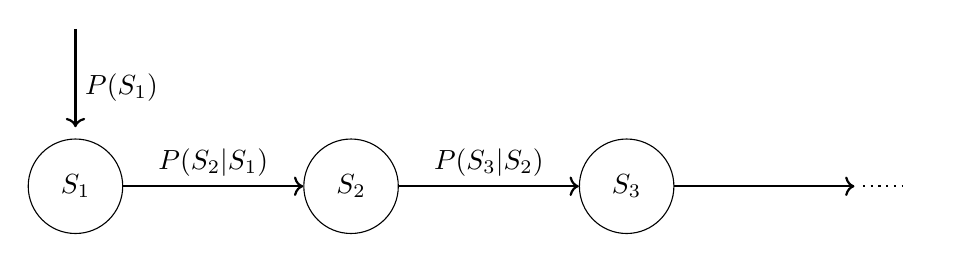
\begin{tikzpicture}[mystate/.style={draw,circle,minimum size=1.2cm}]
        
        %circle
        %\draw [thick] (-3.5,-1.6) circle [radius=0.6];
        %\draw [thick] (-0.9,-1.6) circle [radius=0.6];
        %\draw [thick] (1.7,-1.6) circle [radius=0.6];
        %\draw [thick] (6.8,-1.6) circle [radius=0.6];
        %\draw [thick] (9.4,-1.6) circle [radius=0.6];
        
        %label state
        \node[mystate] (A) at (-3.5,0) {$S_1$};
        \node[mystate] (B) at (0,0) {$S_2$};
        \node[mystate] (C) at (3.5,0) {$S_3$};
        \node[minimum size=1.2cm] (C')at (7,0){};
        
        %horizontal arrow
        \draw [->, thick] (A) -- (B) node[midway, above] {$P(S_2|S_1)$};
        \draw [->, thick] (B) -- (C) node[midway, above] {$P(S_3|S_2)$};
        \draw [->, thick] (C) -- (C') node[midway, above] {};
        
        
        %dots
        \draw [thick, dotted] (6.5,0) -- (7,0);
        
        
        
        %vertical arrow
        \draw [->, thick] (-3.5,2) --(-3.5,.75);
        
        \node [right] at (-3.5,1.25) {{$P(S_1)$}};
        \end{tikzpicture}
        \end{center}
        \end{figure}
\end{frame}

%------------------------------------------------

\begin{frame} {Hidden Markov Model}
    \begin{figure}
        \begin{center}
        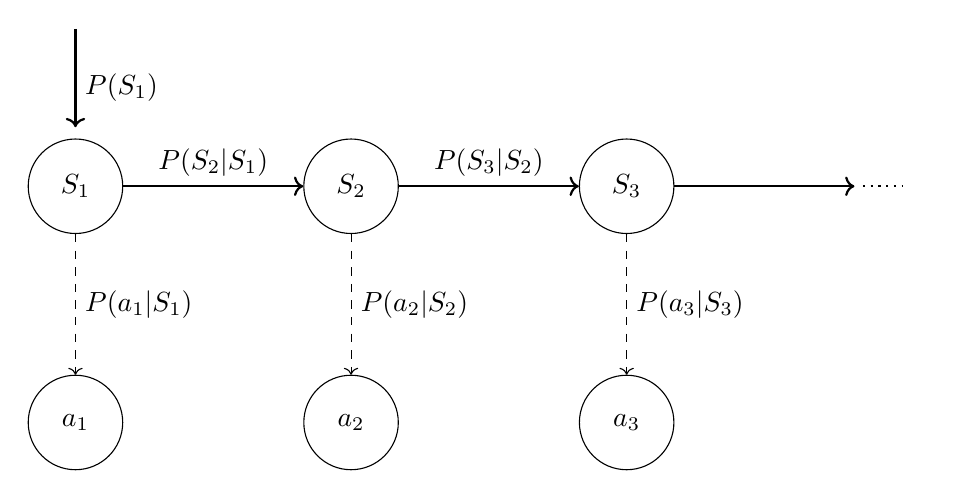
\begin{tikzpicture}[mystate/.style={draw,circle,minimum size=1.2cm}]
        
        %circle
        %\draw [thick] (-3.5,-1.6) circle [radius=0.6];
        %\draw [thick] (-0.9,-1.6) circle [radius=0.6];
        %\draw [thick] (1.7,-1.6) circle [radius=0.6];
        %\draw [thick] (6.8,-1.6) circle [radius=0.6];
        %\draw [thick] (9.4,-1.6) circle [radius=0.6];
        
        %label state
        \node[mystate] (A) at (-3.5,0) {$S_1$};
        \node[mystate] (B) at (0,0) {$S_2$};
        \node[mystate] (C) at (3.5,0) {$S_3$};
        \node[minimum size=1.2cm] (C')at (7,0){};

        \node[mystate] (A1) at (-3.5,-3) {$a_1$};
        \node[mystate] (B1) at (0,-3) {$a_2$};
        \node[mystate] (C1) at (3.5,-3) {$a_3$};
        
        %horizontal arrow
        \draw [->, thick] (A) -- (B) node[midway, above] {$P(S_2|S_1)$};
        \draw [->, thick] (B) -- (C) node[midway, above] {$P(S_3|S_2)$};
        \draw [->, thick] (C) -- (C') node[midway, above] {};

        \draw [->, dashed] (A) -- (A1) node[midway, right] {$P(a_1|S_1)$};
        \draw [->, dashed] (B) -- (B1) node[midway, right] {$P(a_2|S_2)$};
        \draw [->, dashed] (C) -- (C1) node[midway, right] {$P(a_3|S_3)$};

        
        
        %dots
        \draw [thick, dotted] (6.5,0) -- (7,0);
        
        
        
        %vertical arrow
        \draw [->, thick] (-3.5,2) --(-3.5,.75);
        
        \node [right] at (-3.5,1.25) {{$P(S_1)$}};
        \end{tikzpicture}
        \end{center}
        \end{figure}
\end{frame}

%------------------------------------------------

\begin{frame}{Notation}
\begin{itemize}
    \item Let i indicate person i where $1 \leq i \leq N$
    \item Let t indicate current time where $1 \leq t \leq T$
    \item  $\textbf{S}_i = \{S_{i1}, S_{i2}, ..., S_{iT}\}$ is the first order Markov chain of latent states for person i and is fully described by $P(S_{i1})$ and $P(S_{it}|S_{it-1})$
    \item $\textbf{a}_i = \{a_{i1}, a_{i2}, ..., a_{iT}\}$ is the vector of observed measures for person i with the following conditional independence assumption: $P(a_{it}|\textbf{S}_i) = P(a_{it}|S_{it})$
\end{itemize}
\end{frame}


%------------------------------------------------
\begin{frame}
\frametitle{MC Notation}
\begin{itemize}
    \item Let $p_{j} = P(S_{i1} = j)$
    \item Let $p_{kj}(it) = P(S_{it} = j|S_{it-1} = k)$
    \item Model $p_{01}(it) = \text{expit}(X_{it}\beta_0)$ and $p_{10}(it) = \text{expit}(X_{it}\beta_1)$
    \item Covariates can be both fixed (age) and time varying (current time of day)
\end{itemize}
\end{frame}

%------------------------------------------------




\begin{frame}{Emission Notation}
\begin{itemize}
\item $S_{it}  = \begin{cases}
    0  & \text{ if person i is awake at time t} \\ 
    1  & \text{ if person i is asleep at time t} \\
\end{cases}$

\item $\delta_{it}  = \begin{cases}
    0  & \text{if } a_{it} = 0 \\ 
    1  & \text{if } a_{it} \neq 0 \\
\end{cases}$
\bigskip

    \item $a_{it}  = \begin{cases}
                    N(\mu_0 + u_i, \sigma^2_0) & \text{if } S_{it}=0 \text{ and } \delta_{it} = 1\\ 
                    0  & \text{if } S_{it}=0 \text{ and } \delta_{it} = 0\\ 
                    N(\mu_1,\sigma^2_1) & \text{if } S_{it}=1 \text{ and } \delta_{it} = 1\\ 
                    0 & \text{if } S_{it}=1 \text{ and } \delta_{it} = 0\\ 
    \end{cases}$
    \smallskip

% \item Where $Z_{j}(S_{it}) = \begin{cases}
%                             1 & \text{if } S_{it} = j \\
%                             0 & \text{otherwise} \\ \end{cases}$

\item Where $\lambda_0 = P(a_{it}=0|S_{it}=0)$ and $\lambda_1 = P(a_{it}=0|S_{it}=1)$
\end{itemize}
\end{frame}

%------------------------------------------------

\begin{frame}{Motivating Example}
\begin{itemize}
    \item Let $\mu_0 = 2$, $\mu_1 = 0$, $\sigma_0^2 = 3$,  and $\sigma_1^2 = 2$.
    \item Suppose $u_i \sim \text{unif}(-1,1)$. Then we might have $u_1 = .8$ and $u_2 = -.7$ 
    \bigskip
    \item For person 1 we observe $a_{1t}  \sim \begin{cases}
                    N(2.8,3)  & \text{if } S_{it}=0 \\ 
                    N(0,2)  & \text{if } S_{it}=1 \\ 
    \end{cases}$
    \bigskip
    \item For person 2 we observe $a_{2t}  \sim \begin{cases}
                    N(1.3,3)  & \text{if } S_{it}=0 \\ 
                    N(0,2)  & \text{if } S_{it}=1 \\ 
    \end{cases}$
\end{itemize}

\end{frame}

%------------------------------------------------
\begin{frame}{Non-Parametric Density Estimation}
\begin{itemize}
    \item Estimate the RE distribution by a discrete RV, $b_i$, with finite number of support points
    \item Discrete distribution puts mass $\pi_l$ on point $r_l$, $P(b_i = r_l) = \pi_l$
\end{itemize}

\centering
\includegraphics[scale = .55]{Support/nonparametricprobdist_plot1.png}

\end{frame}

%------------------------------------------------
\begin{frame}{Goals}
\begin{itemize}
    \item We have activity data and want to reconstruct the sleep/wake cycle as it has important health implications
    \item When estimating the sleep/wake cycle do we need to model the random effect? What happens if we ignore it and fit a standard HMM instead?
    \item If we include the RE, how many support points do we need? 
\end{itemize}

\end{frame}

%------------------------------------------------

\iffalse
\begin{frame}{Likelihood}
\begin{align*}
f(\textbf{a}|\theta) = \prod_{i=1}^n \int_U \sum_{{s_1}\cdots{s_T}} \biggr[ p_{s_1} \prod_{t=2}^T p_{s_{t-1}s_t}(it) \prod_{t=1}^T \lambda_{s_t}^{\delta_{it}} \big[(1-\lambda_{s_t})P(a_{it}|S_{it}=s_t,u_i)\big]^{1-\delta_{it}}\biggr] dH(u_i)

f(\textbf{a}|\theta) &= \prod_{i=1}^n\int_U\sum_{{s_1}\cdots{s_T}} \biggr[ P(s_{1})\prod_{t=2}^TP(s_{t}|s_{t-1}) \times \prod_{t=1}^T P(a_{it}|s_{t},u_i) \biggr] dH(u_i) \\
\bigskip
&= \prod_{i=1}^n\sum_{l=1}^L\sum_{{s_1}\cdots{s_T}} \biggr[ P(s_{1})\prod_{t=2}^TP(s_{t}|s_{t-1}) \times \prod_{t=1}^T P(a_{it}|s_{t},b_l) \biggr] \pi_l\\
\end{align*}
\end{frame}
\fi

%------------------------------------------------

\begin{frame}{Likelihood}
\begin{alignat*}{2}
f(\textbf{a}|\theta) & = \prod_{i=1}^n && \int_U \sum_{{s_1}\cdots{s_T}} \biggr[ p_{s_1} \prod_{t=2}^T p_{s_{t-1}s_t}(it) \\ 
& && \prod_{t=1}^T \lambda_{s_t}^{\delta_{it}} \big[(1-\lambda_{s_t})P(a_{it}|S_{it}=s_t,u_i)\big]^{1-\delta_{it}}\biggr] dH(u_i)\\
&= \prod_{i=1}^n && \sum_{l=1}^L \sum_{{s_1}\cdots{s_T}}\biggr[ p_{s_1} \prod_{t=2}^T p_{s_{t-1}s_t}(it)\\
& && \prod_{t=1}^T \lambda_{s_t}^{\delta_{it}} \big[(1-\lambda_{s_t})P(a_{it}|S_{it}=s_t,b_i=r_l)\big]^{1-\delta_{it}} \biggr] \pi_l\\
\end{alignat*}
\end{frame}

%------------------------------------------------




%Define Q(theta|theta) as the expected value of the log likelihood function of theta with respect to the current conditional distribution of S  given X and the current estimates of the parameters

%The EM or expectation-maximization algorithm is an approach for performing maximum likelihood estimation in the presence of latent variables. It does this by first estimating the values for the latent variables in the e step, then optimizing the model in the m step. these two steps are repeated until convergence.

\begin{frame}{EM Algorithm }
\begin{itemize}
    \item E-step: $Q(\theta|\theta^{(t)}) = E_{\textbf{S}|\textbf{a},\theta^{(t)}}[\text{log }L(\theta ;\textbf{a},\textbf{S})]$
    \item M-step: $\theta^{(t+1)} = \text{arg max}_\theta \text{ } Q(\theta|\theta^{(t)}) $
\end{itemize} 

\end{frame}

%------------------------------------------------

\begin{frame}{Complete Data}

\begin{itemize}
    \item What if we knew \textbf{S} and \textbf{b}
    \bigskip
    \begin{adjustwidth}{-2.5em}{-2.5em}
    $\begin{aligned}
        f(\textbf{a},&\textbf{S}, \textbf{b} | \theta)  = \\
        &\prod_{i=1}^n \prod_{j=0}^1 p_j^{I(S_{i1}=j)} \\
    & \prod_{i=1}^n \prod^T_{t=2} \prod_{k=0}^1 \prod_{j=0}^1  
        p_{kj}(it)^{I(S_{it-1}=k,S_{t}=j)} \\ 
    & \prod_{i=1}^n\prod_{l=1}^L \prod^T_{t=1}\prod_{j=0}^1 \biggr[
        \lambda_j^{\delta_{ij}} \big[(1-\lambda_j)P(a_{it}|S_{it}=j,b_i=r_l)\big]^{1-\delta_{ij}}
        \biggr]^{I(S_{it}=j,b_i=r_l)} \\
    & \prod_{i=1}^n\prod_{l=1}^L \pi_l^{I(b_i=r_l)}
    \end{aligned}$
    \end{adjustwidth}
    \bigskip


\end{itemize}

\end{frame}

%------------------------------------------------
\begin{frame}[shrink=5]{Expectation of Complete Data Log Likelihood}
\framesubtitle{E Step}

\begin{itemize}
    \item Replace $f(\textbf{a},\textbf{S}, \textbf{b} | \theta)$ with E$\big[\text{log f}(\textbf{a},\textbf{S}, \textbf{b} | \theta) | \textbf{a},\theta\big]$ \bigskip
    \begin{adjustwidth}{-3.5em}{-3em}
    $\begin{aligned}
        \ell = & E\big[\text{log f}(\textbf{a},\textbf{S}, \textbf{b} | \theta) | \textbf{a},\theta\big]\\
    = & \sum_{i=1}^n\sum_{j=0}^1P(S_{i1}=j|\textbf{a})\text{log }p_j + \\
    & \sum_{i=1}^n \sum^T_{t=2} \sum_{k=0}^1 \sum_{j=0}^1 
        P(S_{it-1}=k,S_{it}=j|\textbf{a})\text{log }p_{kj}(it) + \\ 
    & \sum_{i=1}^n \sum_{l=1}^L \sum^T_{t=1}\sum_{j=0}^1 P(S_{it}=j,b_i=r_l|\textbf{a}) \biggr[\delta_{it}\text{log }\lambda_j +  \\
    & \phantom{\sum_{i=1}^n \sum^T_{t=2} \sum_{k=0}^1 \sum_{j=0}^1} 
    (1-\delta_{ij})\text{log}\Big((1-\lambda_j)P(a_{t}|S_{it}=j, b_i=r_l) \Big)\biggr]+ \\
    &  \sum_{i=1}^n \sum_{l=1}^L P(b_i=r_l|\textbf{a}) \text{log }\pi_l  
    \end{aligned}$
    \end{adjustwidth}



\end{itemize}

\end{frame}

%------------------------------------------------


% \begin{frame}{RE Likelihood}

% \begin{itemize}
%     \item Focus on part of likelihood dealing with the random effect \bigskip
%     \begin{adjustwidth}{-2em}{-1em}
%     $\begin{aligned}
%         &\sum_{i=1}^n \sum_{l=1}^L \sum^T_{t=1} P(S_{it} =0,b_i=r_l|\textbf{a}) \text{log}P(a_{it}|S_{it}=0, b_i=r_l) + \\
%         &\sum_{i=1}^n \sum_{l=1}^L P(b_i=r_l|\textbf{a})\text{log }\pi_l 
%     \end{aligned}$
%     \end{adjustwidth}
%     \bigskip
%     \item $P(b_i=r_l|\textbf{a})$ is the probability that individual i belongs to component l
%     \smallskip
%     \item $P(S_{it} =0,b_i=r_l|\textbf{a})$ is the probability that individual i belongs to component l and awake at time t 
%     \smallskip
%     \item $\text{log}P(a_{it}|S_{it}=0, b_i=r_l) = \text{log N}(a_{it}| \mu = \mu_0 + r_l, \sigma^2 = \sigma_0^2)$


% \end{itemize}

% \end{frame}

%------------------------------------------------



% \begin{frame}{Forward-Backward Algorithm \cite{Baum1970}}
% \begin{itemize}
%     \item $\alpha_{it}(j,r_l) = P(a_{i1}, ..., a_{it}, S_{it} = j | b_i=r_l)$
% \end{itemize}

% \[ \alpha_{it}(j,r_l) = \begin{cases}
%     \delta_{j}f(a_{i1}|S_{i1}=j,r_l)& \text{if } t = 1 \\
%     \sum_{k=0}^1 \alpha_{it-1}(k,b_l)\delta_{kj}f(a_{it}|S_{it}=j,b_i=r_l) & \text{if } t > 1\\
% \end{cases}\]
% \bigskip
% \begin{itemize}
%     \item $\beta_{it}(j,r_l) =  P(a_{it+1}, ..., a_{iT} | S_{it} = j,b_i=r_l)$
% \end{itemize}

% \[ \beta_{it}(j,r_l) = \begin{cases} 
%     1 & \text{if } t = n \\
%     \sum_{k=0}^1\delta_{jk}f(a_{it+1}|S_{it+1}=k,b_i=r_l)\beta_{it+1}(k,r_l)& \text{if } t < n \\
% \end{cases}\] 


% \end{frame}
%------------------------------------------------


\begin{frame}{Emission Closed Form Solutions}
\framesubtitle{M Step}
\begin{itemize}

    \item $\hat{p_j}  = \frac{\sum^n_{i=0} P(S_{i1}=0|\textbf{a})}{n}$
    
    \item $\hat{\lambda_j}  = \frac{\sum^n_{i=0} \sum_{t=1}^T P(S_{it}=j|\textbf{a})\delta_{it}}{\sum^n_{i=0} \sum_{t=1}^TP(S_{it}=j|\textbf{a})}$

    \item $\hat{\mu_0} +\hat{r_l} = \frac{\sum_{i=1}^n \sum_{t=1}^T a_{it}P(S_{it}=0,b_{i}=r_l|\textbf{a})}
    {\sum_{i=1}^n \sum_{t=1}^T P(S_{it}=0,b_{i}=r_l|\textbf{a})}$
    \item $\hat{\sigma}_0^2 = \frac{\sum_{i=1}^n \sum_{l=1}^L \sum_{t=1}^T (1-\delta_{it})(a_{it}-\nu_l)^2 P(S_{it}=0,b_{i}=r_l|\textbf{a})} {\sum_{i=1}^n \sum_{l=1}^L \sum_{t=1}^T (1-\delta_{it}) P(S_{it}=0,b_{i}=r_l|\textbf{a})}$
    \item $\hat{\pi_l} = \sum_{i = 1}^n \frac{P(b_i = r_l)}{n}$
\end{itemize} 

    
\end{frame}




%------------------------------------------------


\begin{frame}{Transition Probability Calculation}
    \begin{itemize}
        \item No closed form solution for the transition probabilities
        \item Recall $p_{01}(it) = \text{expit}(X_{it}\beta_0)$ and $p_{10}(it) = \text{expit}(X_{it}\beta_1)$
        \item Single step of Newton-Raphson in each EM step
        \item $\beta_{j}^* = \beta_{j} - (\frac{\partial^2\ell}{\partial \beta_{j}^2})^{-1} \frac{\partial\ell}{\partial \beta_{j}}$, where $\beta_{j}$ is our current estimate and $\beta_{j}^*$ is the updated estimate
    \end{itemize}
    
\end{frame}

%------------------------------------------------

\begin{frame}{Forward-Backward Algorithm}
\begin{itemize}
    \item $\alpha_{it}(j,r_l) = P(a_{i1}, ..., a_{it}, S_{it} = j | b_i=r_l)$
    \smallskip
    \item $\beta_{it}(j,r_l) =  P(a_{it+1}, ..., a_{iT} | S_{it} = j,b_i=r_l)$
\end{itemize} 

\bigskip
\bigskip

$\begin{aligned}
    P(b_{i}=r_l|\textbf{a}) & = \frac{P(\textbf{a}|b_{i}=r_l)P(b_{i}=r_l)}{P(\textbf{a})} = 
    \frac{\sum_{j=0}^1 \alpha_{it}(j,r_l)\beta_{it}(j,r_l)\pi_l }
    {\sum_{j=0}^1\sum_{l=1}^L \alpha_{it}(j,r_l)\beta_{it}(j,r_l)\pi_l } 
\end{aligned}$

\bigskip
\bigskip

$\begin{aligned}
    P(S_{it}=0,b_{i}=r_l|\textbf{a}) & = \frac{P(\textbf{a},S_{it}=0|b_{i}=r_l)P(b_{i}=r_l)}{P(\textbf{a})} \\
    & = \frac{\alpha_{it}(0,r_l)\beta_{it}(0,r_l)\pi_l }
    {P(\textbf{a})}
\end{aligned}$

\end{frame}



%------------------------------------------------

\begin{frame}{Simulation Study}
\begin{enumerate}
    \item Generated a sequence of MC states $\{S_{i1}, ..., S_{iT}\}$ corresponding to the wake/sleep state of person i at time t
    \item Draw a random effect for person i from its density, $u_i \sim H$. H needs to be a valid distribution centered at 0
    \item Simulate fake observed activity data
    \begin{itemize}
        \item $a_{it} \sim \begin{cases}
                    N(2+u_i,3)  & \text{if } S_{it}=0 \\ 
                    N(0,2)  & \text{if } S_{it}=1 \\ 
    \end{cases}$
    \end{itemize}
    \item Estimate parameters, varying number of support points, underlying continuous RE distribution, and sample size
    \item Use the Viterbi algorithm to create the most likely sequence of wake/sleep states using the estimated parameters
    \item Compare the estimated wake/sleep sequence with the true simulated wake/sleep sequence
\end{enumerate} 

    
\end{frame}


%------------------------------------------------
\begin{frame}{Models}
    \begin{itemize}
        \item Shared HMM
        \item Individual HMM
        \item Mixed HMM with 2-8 support points
        \item Initial, transition, and sleep emission parameters are shared across all individuals for each model
    \end{itemize}
\end{frame}
%------------------------------------------------
\begin{frame}{Distributions}
\centering
\includegraphics[scale = .45]{Support/REdist.png}
\end{frame}


%------------------------------------------------

\begin{frame}{Overall Accuracy}
\centering
\includegraphics[scale = .6]{Support/NestedLoopAcc.png}

    
\end{frame}


%------------------------------------------------
\begin{frame}{Overall Accuracy Discussion}
    \begin{itemize}
        \item Shared HMM is consistently the worst
        \item Individual HMM preforms well with longer follow-up
        \item Increasing the number of support points increases accuracy with diminishing returns
    \end{itemize}
\end{frame}
%------------------------------------------------

\begin{frame}{Sensitivity and Positive Predictive Value (PPV)}
\centering
\includegraphics[scale = .39]{Support/NestedLoopSP.png}

    
\end{frame}


%------------------------------------------------
\begin{frame}{Sensitivity and PPV Discussion}
    \begin{itemize}
        \item Shared HMM and MHMM2 predict sleep in situations that are uncertain (low wake sensitivity, and high wake PPV)
        \item Increasing number of support points or using an individual HMM more accurately predicts these indeterminate cases 
    \end{itemize}
\end{frame}
%------------------------------------------------


\begin{frame}{Transition Residuals}
\centering
\includegraphics[scale = .39]{Support/NestedLoopTran.png}

    
\end{frame}


%------------------------------------------------



\begin{frame}{Mixing Proportion vs Wake Activity Cluster}
    \centering
    \includegraphics[scale = .6]{Support/clustmeanmix.png}
    
        
    \end{frame}
    
    
    %------------------------------------------------
\begin{frame}{Simulation Conclusions}
\begin{itemize}
    \item Shared HMM consistently had the lowest accuracy, most biased, and was influenced the most by choice of H
    \item Individual HMM was very accurate for longer follow up, but may be biased for transition estimation depending on H
    \item MHMM with many support points was consistently the most accurate and least biased 
\end{itemize}

    
\end{frame}


%------------------------------------------------
    
    

\end{document}
